\chapter{Results}

\section{Automatic Evaluation}

\begin{table}
\begin{center}
\small
\begin{tabular}{lcc}
\textbf{Model}        	& \textbf{Dev}	& \textbf{Test}	\\
\hline
Transformer base    					& 37.28 & 36.66 \\
Transformer relative					& 37.23 & 37.02 \\
\hline
(base) + tree dist., max 5				& 35.47 & 33.13 \\
(base) + tree dist., max 20				& 34.45 & 35.50 \\
(base) + tree traversal					& 35.21 & 35.80 \\
(tree\_5) + abs. seq					& 37.67 & \textbf{37.49} \\
(relative) + tree dist., max 20			& 37.15 & \textbf{37.55} \\
(relative) + tree traversal				& 38.22 & \textbf{37.80} \\
\hline
(base) + spec. POS						& 36.97 & 36.65 \\
(base) + spec. dep. rel.				& 37.81 & 36.93\\
(relative) + spec. dep. rel.			& 37.53 &  \textbf{37.72} \\
\end{tabular}
\end{center}
\caption{Enriching encoder results}
\end{table}


\cref{tab:trans_depparse_res} shows the effect of choosing self-attention weight from different layers in the Transformer's encoder.

\begin{table}
\centering
\small
\vspace{2ex}
  \begin{tabular}{lcc|cc}
    &  \multicolumn{2}{c}{\textbf{BLEU}} & \multicolumn{2}{|c}{\textbf{UAS}} \\
    & \textbf{Dev} & \textbf{Test} & \textbf{Dev} & \textbf{Test} \\
    \hline
    Transformer & 37.28 & 36.66 & -- & -- \\
    \hline
    Parse layer 0 & 36.95 & 36.60 & 81.39 & 82.85 \\
    Parse layer 1 & \textbf{38.51} & \textbf{38.01} & 90.17 & 90.78 \\
    Parse layer 2 & 38.50 & 37.87 & 91.31 & 91.18 \\
    Parse layer 3 & 38.37 & 37.67 & 91.43 & 91.43 \\
    Parse layer 4 & 37.86 & 37.60 & \textbf{91.65} & \textbf{91.56} \\
    Parse layer 5 & 37.63 & 37.67 & 91.44 & 91.46 \\
  \end{tabular}
  \caption{Joint model results in translation (BLEU) and parsing (UAS) on automatically annotated data.}
  \label{tab:trans_depparse_res}
\end{table}

\begin{table}
\begin{center}
\small
\begin{tabular}{lcc}
\textbf{Model}        	& \textbf{de2cs}	& \textbf{cs2en}	\\
\hline
Transformer base    & 13.96	&  36.66 \\
Our joint model		& 14.27	&  38.01 \\
\end{tabular}
\end{center}
\caption{BLEU scores on test set for translation task.}
\label{multidec-results}
\end{table}


\cref{multidec-results} presents the experiment result, in which our proposed
model outperformed the baseline in the translation task.

More importantly, the choice of the head from one layer that will serve as the
dependency parser is arbitrary, but selecting which layer matters. There are six
layers in the encoder. \cref{tab:trans_depparse_res} shows the result of both
tasks when different layers in the encoder is chosen to dedicate one of its
self-attention heads to be the dependency matrix.

It is apparent from this table that layer 0 (the first layer) is a too early
stage for both task. This layer is challenging because the current
self-attention mechanism purely compares between input word embeddings, which
may be more semantically useful than syntactically. On the other hand, layer
1 and 2 perform well on the parsing task, and are the bests for the translation
task. A possible explanation is that they are not extremely premature as layer
0, yet not too high in the encoder, hence allow higher layers to freely learn
more information. The highest layers are the best for the parsing task while
still be able to maintain good translation performance. When reaching these
layers, the encoder has already learned a good presentation for each words,
which is very informative for the parsing task.

We also compared our joint model on gold annotated treebanks.

In addition to the automatically annotated test set, we also evaluated our model on the gold evaluation sets
from UD 2.0 for German and from PDT 2.5 for Czech.

As referential parser we use UDPipe for German, the one which supervised our model.
Our system gains similar UAS performance. It should be noted that we used
the supervision by UDPipe in a non-standard way. Our system (and referential
parser) take raw word tokens on input, while
UDPipe is designed to segment multi-word tokens, such as \textit{zum}, into
syntactic words, as \textit{zu dem}, each of which are single nodes in tree.
For Czech we report the score of winner in
CoNLL Shared Task 2007 \parcite{connl2007}, the latest available evaluation 
on same data. We expect that state-of-the-art is higher nowadays. The
limitation of our model may be shared decoder and potentially inaccurate
automatically annotated training data.

\cref{multidec-results-parse} shows that our model achieved good results in compare to the baseline model on those datasets, even though ours was trained using synthetic data.

\begin{table}
\begin{center}
\small
\begin{tabular}{lcc}
\textbf{Model}        	& \textbf{de}	& \textbf{cs}	\\
\hline
% Stanford \citep{dozat-qi-manning:2017:K17-3} & 84.10 & -- \\
UDPipe 1.2 (de) 		& 74.27 & -- \\ % UAS: 74.15, LAS: 68.61 in CoNLL Shared task 2017
Nakagawa (2007) 		& -- &  86.28 \\
Our joint model			& 76.48	&  82.53 \\
\end{tabular}
\end{center}
\caption{UAS on gold annotated test sets for parsing task.}
\label{multidec-results-parse}
\end{table}

\section{Training Speed}

As proven that the NMT model has already captured the dependency links, our joint models, without the complex sub-model for parsing, were trained in a comparable time with the transformer\_base. Training time (including internal evaluation each 1000 steps) to reach 250,000 steps for the transformer\_base is 1 days, 3 hours, 48 minutes. While our joint models vary from 1 days, 4 hours, 40 minutes to 1 days, 5 hours, 20 minutes on a single GPU NVIDIA GTX 1080Ti.

While having achieved the results discussed above, the training cost for our multi-task model is comparable to only translating Transformer. The training time (including internal evaluation each 1000 steps) to reach 250k steps for the \texttt{transformer\_base} was 1 days, 3 hours, 48 minutes. While our joint models varied from 1 days, 4 hours, 40 minutes to 1 days, 5 hours, 20 minutes on a single GPU Nvidia GTX 1080Ti.

\section{Self-Attention Analysis}

\begin{figure}
	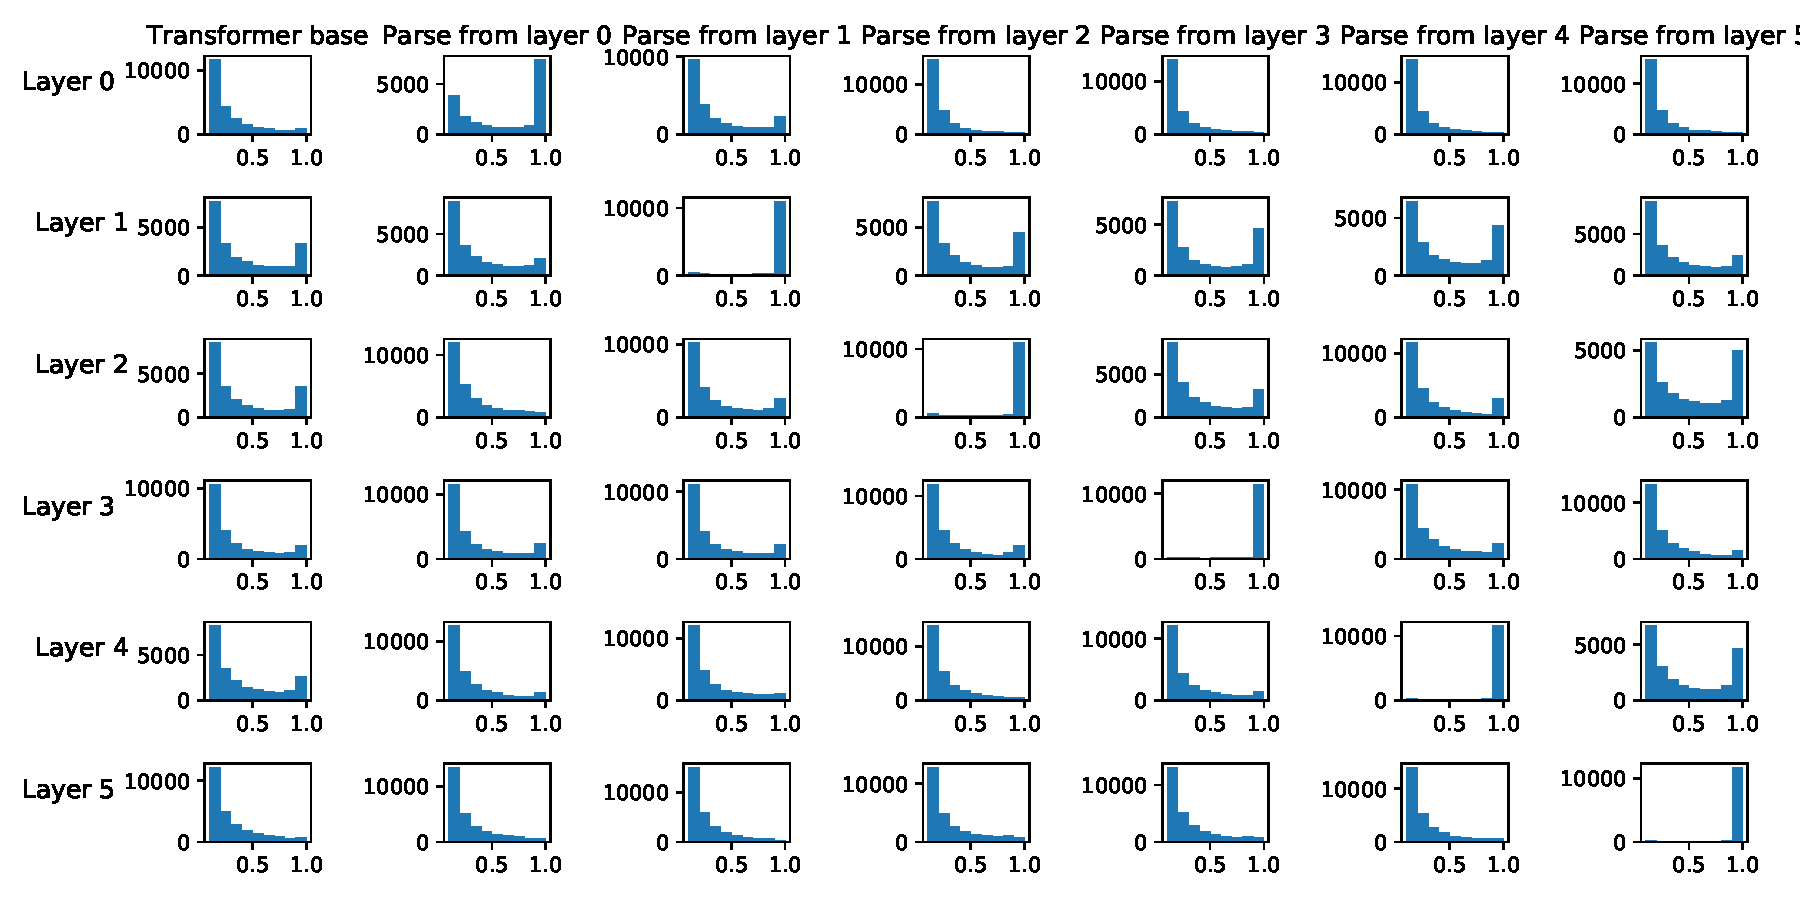
\includegraphics[width=\textwidth]{img/att_dist}
    \caption{Histogram of normalized self-attention weights in the encoder.}
    \label{fig:att_dist}
\end{figure}

\begin{figure}
    \centering
	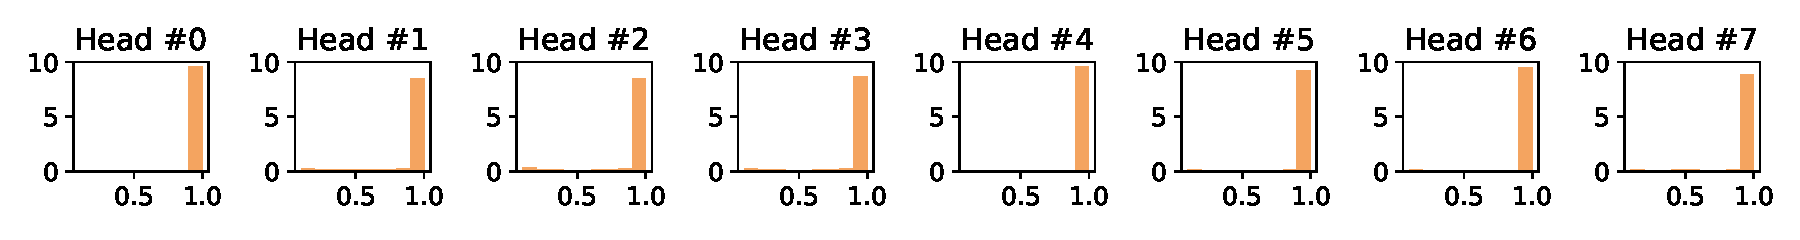
\includegraphics[width=0.8\textwidth]{img/att_dist_4}
    \caption{Histogram of self-attention weights in the encoder's layer 4 when parsing from layer 4.}
    \label{fig:att_dist_4}
\end{figure}

Figure \ref{fig:att_dist} presents the behavior of self-attention mechanism in each layers of our experimented models for the first 100 sentences in the test set. The bin $[0.0,0.1)$ has been removed for a clearer comparison because most of the self-attention weights fall into this trivial bin. As can be seen from the figure, the layers in which the model performed parsing display a very sharp attention, i.e. for each head, a word only attend to only one or two other words. This behavior exists in every of our multi-task models, except the "Parse from layer 0". As mentioned in \XXX{section results}, this exception model performed badly on both tasks, hence, our hypothesis is that this sharpness or our restricted self-attention helped the model to perform better.

It is also important to note that one can argue because we used the self-attention weight to predict dependency heads, it is normal for the head to display this behavior. However, from the experiments, not only the chosen head, but the other heads in the same layer also learned this behavior, which is shown in \cref{fig:att_dist_4} (bin $[0.0,0.1)$ was also removed).
